\documentclass[12pt,a4paper]{article}

% --- Настройка языка и шрифтов для LuaLaTeX ---
\usepackage{fontspec}
\defaultfontfeatures{Ligatures=TeX,Scale=MatchLowercase}

\setmainfont{Alice-Regular}[
    Path=font/,
    Extension=.ttf,
    BoldFont = Alice-Regular,
    ItalicFont = Alice-Regular,
    BoldItalicFont = Alice-Regular,
    BoldFeatures = {FakeBold=1.6},
    ItalicFeatures = {FakeSlant=0.2},
    BoldItalicFeatures = {FakeBold=1.6,FakeSlant=0.2}
]

\newfontfamily\cyrillicfont{Alice-Regular}[
    Path=font/,
    Extension=.ttf,
    BoldFont = Alice-Regular,
    ItalicFont = Alice-Regular,
    BoldItalicFont = Alice-Regular,
    BoldFeatures = {FakeBold=1.6},
    ItalicFeatures = {FakeSlant=0.2},
    BoldItalicFeatures = {FakeBold=1.6,FakeSlant=0.2}
]

\usepackage{polyglossia}
\setmainlanguage{russian}
\setsansfont{TeX Gyre Heros}
\setmonofont{TeX Gyre Cursor}

\usepackage{graphicx}        					% Графика
\usepackage{amsmath, amsfonts, amssymb, amsthm}	% Математика
\usepackage{mathtools}
\usepackage{chemfig}
\usepackage[version=4,arrows=pgf-filled,
            textfontname=sffamily,
            mathfontname=mathsf]{mhchem}
\usepackage[protrusion=false]{microtype}       % Микротипографика
\usepackage{braket} 						% Braket нотация для квантовой механики
\usepackage{unicode-math} 					% Современный пакет для математики в LuaLaTeX
\usepackage{longtable}       				% Таблицы с разрывом страниц
\usepackage{tikz}           				% Рисование
\usepackage[europeanresistors]{circuitikz}	% Рисование электрических схем в европейском стиле
\usepackage{listings}						% Для отображения кода
\usepackage{tabularx}       				% Для таблиц во всю ширину
\usepackage{array}		  					% Для расширенных возможностей таблиц
\usepackage{float}          				% Для точного позиционирования фигур
\usepackage{pgfplots}                          % Для построения графиков
\usepackage{caption}                           % Для настройки подписей к рисункам и таблицам
\usepackage{xfp}                               % Для вычислений в LaTeX
\usepackage{luacode}                           % Для выполнения Lua-кода в документе    
\pgfplotsset{compat=1.18}
\usepackage[paper=letterpaper,
            top=20mm,
            bottom=20mm,
            left=10mm,
            right=10mm,
            footskip=0.4in 
]{geometry}

\usetikzlibrary{arrows.meta}

% --- Колонтитулы ---
\usepackage{fancyhdr}
\pagestyle{fancy}
\fancyhf{}

% --- Теоремы и окружения ---
\theoremstyle{plain}
\newtheorem{theorem}{Theorem}[section]
\newtheorem{lemma}[theorem]{Lemma}
\newtheorem{proposition}[theorem]{Proposition}
\newtheorem{corollary}[theorem]{Corollary}

\theoremstyle{definition}
\newtheorem{definition}[theorem]{Definition}

\theoremstyle{remark}
\newtheorem{remark}[theorem]{Remark}

\numberwithin{equation}{section}


\renewcommand{\headrulewidth}{0.4pt}
\renewcommand{\footrulewidth}{0.4pt}
\renewcommand\lstlistingname{Исходный код}

\lstdefinestyle{main}{
	backgroundcolor=\color{gray!8},   
	commentstyle=\color{green!50!black},
	keywordstyle=\color{blue!80!black},
	numberstyle=\small\color{darkgray},
	stringstyle=\rmfamily\color{orange!90!black},
	basicstyle=\ttfamily\small,
	breakatwhitespace=false,         
	breaklines=true,                   
	keepspaces=true,                 
	numbers=left,                    
	numbersep=8pt,                  
	showspaces=false,                
	showstringspaces=false,
	showtabs=false,                  
	tabsize=4
}	

\lstset{style=main}

\newcolumntype{C}{>{\centering\arraybackslash}X}
\renewcommand{\arraystretch}{1.25}

\begin{luacode*}
    data = require("data")
    include = require("include")
    handle = require("handle")
\end{luacode*}

\begin{document}

\section{\large\textnormal{Рассчитать значения встроенных потенциалов в эмиттере и базе при заданных по варианту значениях $N_\text{э}$ и $N_\text{б}$ (Si, $T = 300\text{ К}$).}}

\begin{figure}[H]
    \centering
    \begin{minipage}[t]{0.3\textwidth}
    \vspace{0em}
    \begin{tabularx}{\textwidth}{|X|}
        \hline
        \multicolumn{1}{|C|}{Дано} \\
        \hline
        полупроводник Si \\ 
        $T = 300$ К \\
        $N_\text{э} = 10^{20}$ см$^{-3}$ ($n^+$-тип) \\
        $N_\text{б} = 10^{18}$ см$^{-3}$ ($p$-тип) \\
        $n_i = 1.45 \cdot 10^{10}$ см$^{-3}$ \\
        $k = 1.381 \cdot 10^{-23}$ Дж/К \\
        $e = 1.602 \cdot 10^{-19}$ Кл \\
        \hline
        \multicolumn{1}{|C|}{Найти} \\
        \hline
        $\varphi_{0\text{э}}$ — ? \\
        $\varphi_{0\text{б}}$ — ? \\
        $\Delta\varphi_{0\text{э}}$ — ? \\
        $\Delta\varphi_{0\text{б}}$ — ? \\
        \hline
    \end{tabularx}

    \vspace{1em}
    Встроенные потенциалы областей относительно собственного полупроводника:
    \begin{equation*}
        \varphi_{0\text{э}} = \frac{kT}{e}\ln\left(\frac{N_\text{э}}{n_i}\right)
    \end{equation*}
    \begin{equation*}
        \varphi_{0\text{б}} = \frac{kT}{e}\ln\left(\frac{N_\text{б}}{n_i}\right)
    \end{equation*}
    Контактный потенциал перехода:
    \begin{equation*}
        \varphi_k = \varphi_{0\text{э}} + \varphi_{0\text{б}}
    \end{equation*}
    Падения потенциала на ОПЗ:
    \begin{equation*}
        \Delta\varphi_{0\text{э}} = \varphi_k \frac{N_\text{б}}{N_\text{э} + N_\text{б}}
    \end{equation*}
    \begin{equation*}
        \Delta\varphi_{0\text{б}} = \varphi_k \frac{N_\text{э}}{N_\text{э} + N_\text{б}}
    \end{equation*}

    \end{minipage}\hfill\begin{minipage}[t]{0.7\textwidth}
        \vspace{0em}
        \begin{tabularx}{\textwidth}{C|}
            \hline
            Решение \\
            \hline
        \end{tabularx}

        \vspace{0.5em}
        \hspace{0.025\textwidth}
        \begin{minipage}[t]{0.95\textwidth}
            Температурный потенциал при $T = 300\text{ К}$:
            \begin{equation*}
                \varphi_T = \frac{kT}{e} = \directlua{
                    tex.sprint("\\frac{"
                               .. include.value_with_mantice(data.k, 2, 0, 0) .. 
                               " \\cdot "
                               .. include.value_with_mantice(data.T, 2, 0, 0) .. 
                               "}{"
                               .. include.value_with_mantice(data.e, 2, 0, 0) .. 
                               "} = "
                               .. include.value_with_mantice(data.phi_T, 2, 0, 0))
                } \text{ В}
            \end{equation*}

            1) Встроенный потенциал в эмиттере ($n^+$-тип):
            \begin{equation*}
                \begin{aligned}
                    \varphi_{0\text{э}} &= \frac{kT}{e}\ln\left(\frac{N_\text{э}}{n_i}\right) = \\
                    &= \directlua{
                        tex.sprint(include.value_with_mantice(data.phi_T, 2, 0, 0) .. 
                                   " \\ln\\left(\\frac{"
                                   .. include.value_with_mantice(data.N_e, 2, 0, 0) .. 
                                   "}{"
                                   .. include.value_with_mantice(data.n_i, 2, 0, 0) .. 
                                   "}\\right) = "
                                   .. include.value_with_mantice(data.phi_0e, 2, 0, 0))
                    } \text{ В}
                \end{aligned}
            \end{equation*}

            2) Встроенный потенциал в базе ($p$-тип):
            \begin{equation*}
                \begin{aligned}
                    \varphi_{0\text{б}} &= \frac{kT}{e}\ln\left(\frac{N_\text{б}}{n_i}\right) = \\
                    &= \directlua{
                        tex.sprint(include.value_with_mantice(data.phi_T, 2, 0, 0) .. 
                                   " \\ln\\left(\\frac{"
                                   .. include.value_with_mantice(data.N_b, 2, 0, 0) .. 
                                   "}{"
                                   .. include.value_with_mantice(data.n_i, 2, 0, 0) .. 
                                   "}\\right) = "
                                   .. include.value_with_mantice(data.phi_0b, 2, 0, 0))
                    } \text{ В}
                \end{aligned}
            \end{equation*}

            Полный контактный потенциал перехода:
            \begin{equation*}
                \varphi_k = \varphi_{0\text{э}} + \varphi_{0\text{б}} = \directlua{
                    tex.sprint(include.value_with_mantice(data.phi_0e, 2, 0, 0) .. 
                               " + " .. 
                               include.value_with_mantice(data.phi_0b, 2, 0, 0) .. 
                               " = " .. 
                               include.value_with_mantice(data.phi_k, 2, 0, 0))
                } \text{ В}
            \end{equation*}

            Падения контактного потенциала на слоях ОПЗ эмиттера и базы:
            \begin{equation*}
                \begin{aligned}
                    \Delta\varphi_{0\text{э}} &= \varphi_k \frac{N_\text{б}}{N_\text{э} + N_\text{б}} = \directlua{
                        tex.sprint(include.value_with_mantice(data.phi_k, 2, 0, 0) .. 
                                   " \\cdot \\frac{" .. 
                                   include.value_with_mantice(data.N_b, 2, 0, 0) .. 
                                   "}{" .. 
                                   include.value_with_mantice(data.N_e, 2, 0, 0) .. 
                                   " + " .. 
                                   include.value_with_mantice(data.N_b, 2, 0, 0) .. 
                                   "} = " .. 
                                   include.value_with_mantice(data.delta_phi_0e, 2, 0, 0))
                    } \text{ В} \\
                    \Delta\varphi_{0\text{б}} &= \varphi_k \frac{N_\text{э}}{N_\text{э} + N_\text{б}} = \directlua{
                        tex.sprint(include.value_with_mantice(data.phi_k, 2, 0, 0) .. 
                                   " \\cdot \\frac{" .. 
                                   include.value_with_mantice(data.N_e, 2, 0, 0) .. 
                                   "}{" .. 
                                   include.value_with_mantice(data.N_e, 2, 0, 0) .. 
                                   " + " .. 
                                   include.value_with_mantice(data.N_b, 2, 0, 0) .. 
                                   "} = " .. 
                                   include.value_with_mantice(data.delta_phi_0b, 2, 0, 0))
                    } \text{ В}
                \end{aligned}
            \end{equation*}

            Ответ: $\varphi_{0\text{э}} = \directlua{
                tex.sprint(include.value_with_mantice(data.phi_0e, 2, 0, 0))
            } \text{ В}$, $\varphi_{0\text{б}} = \directlua{
                tex.sprint(include.value_with_mantice(data.phi_0b, 2, 0, 0))
            } \text{ В}$ (падения на ОПЗ: $\Delta\varphi_{0\text{э}} = \directlua{
                tex.sprint(include.value_with_mantice(data.delta_phi_0e, 2, 0, 0))
            } \text{ В}$, $\Delta\varphi_{0\text{б}} = \directlua{
                tex.sprint(include.value_with_mantice(data.delta_phi_0b, 2, 0, 0))
            } \text{ В}$).
    \end{minipage}\end{minipage}
\end{figure}

\pagebreak

\section{\large\textnormal{Дан переход ($n^+\text{-}p$). Тип и концентрации примеси ($N_\text{э}$ и $N_\text{б}$) перехода заданы по варианту. \\
Задание: \\
- нарисовать переход, выделить нейтральные области и ОПЗ, \\
- указать эмиттер и базу, \\
- указать тип основных носителей в эмиттере и базе, \\
- указать тип неосновных носителей в эмиттере и базе.}}

\begin{figure}[H]
    \centering
    \begin{minipage}[t]{0.3\textwidth}
    \vspace{0em}
    \begin{tabularx}{\textwidth}{|X|}
        \hline
        \multicolumn{1}{|C|}{Дано} \\
        \hline
        Тип перехода: $n^+\text{-}p$ \\
        $N_\text{э} = 10^{20}$ см$^{-3}$ ($n^+$-тип) \\
        $N_\text{б} = 10^{18}$ см$^{-3}$ ($p$-тип) \\
        \hline
        \multicolumn{1}{|C|}{Найти} \\
        \hline
        Схему перехода \\
        Тип областей \\
        Основные носители \\
        Неосновные носители \\
        \hline
    \end{tabularx}

    \vspace{1em}
    Переход $n^+\text{-}p$ резкий асимметричный ($N_\text{э} \gg N_\text{б}$):
    \begin{equation*}
        \frac{l_n}{l_p} = \frac{N_\text{б}}{N_\text{э}} = 10^{-2}
    \end{equation*}
    Вследствие резкой асимметрии ОПЗ практически целиком сосредоточена в слаболегированной базе ($l_p \approx l_0$).
    \end{minipage}\hfill\begin{minipage}[t]{0.7\textwidth}
        \vspace{0em}
        \begin{tabularx}{\textwidth}{C|}
            \hline
            Решение \\
            \hline
        \end{tabularx}

        \vspace{0.5em}
        \hspace{0.025\textwidth}
        \begin{minipage}[t]{0.95\textwidth}
            \centering
            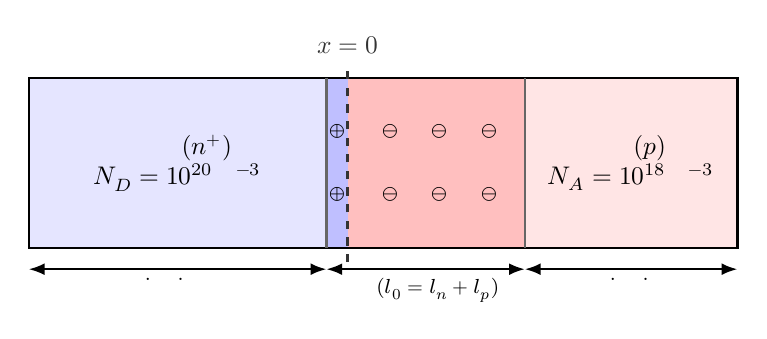
\begin{tikzpicture}[scale=0.9, every node/.style={scale=0.92}]
                % Emitter neutral
                \fill[blue!10] (-4.5,-1.2) rectangle (-0.3,1.2);
                % Emitter SCR
                \fill[blue!25] (-0.3,-1.2) rectangle (0,1.2);
                % Base SCR
                \fill[red!25] (0,-1.2) rectangle (2.5,1.2);
                % Base neutral
                \fill[red!10] (2.5,-1.2) rectangle (5.5,1.2);

                % Border
                \draw[thick] (-4.5,-1.2) rectangle (5.5,1.2);
                % Metallurgical junction
                \draw[very thick, dashed, black!80] (0,-1.4) -- (0,1.4) node[above] {$x = 0$};
                % SCR boundaries
                \draw[thick, black!60] (-0.3,-1.2) -- (-0.3,1.2);
                \draw[thick, black!60] (2.5,-1.2) -- (2.5,1.2);

                % Charges in SCR
                \node at (-0.15,0.45) {\footnotesize $\oplus$};
                \node at (-0.15,-0.45) {\footnotesize $\oplus$};
                \node at (0.6,0.45) {\footnotesize $\ominus$};
                \node at (0.6,-0.45) {\footnotesize $\ominus$};
                \node at (1.3,0.45) {\footnotesize $\ominus$};
                \node at (1.3,-0.45) {\footnotesize $\ominus$};
                \node at (2.0,0.45) {\footnotesize $\ominus$};
                \node at (2.0,-0.45) {\footnotesize $\ominus$};

                % Region labels
                \node[align=center] at (-2.4,0) {\textbf{Эмиттер} ($n^+$)\\ $N_D = 10^{20}\text{ см}^{-3}$};
                \node[align=center] at (4.0,0) {\textbf{База} ($p$)\\ $N_A = 10^{18}\text{ см}^{-3}$};

                % Dimension brackets
                \draw[{Latex[length=2mm]}-{Latex[length=2mm]}, thick] (-0.3,-1.5) -- (2.5,-1.5) 
                    node[midway, below] {\footnotesize ОПЗ ($l_0 = l_n + l_p$)};
                \draw[{Latex[length=2mm]}-{Latex[length=2mm]}, thick] (-4.5,-1.5) -- (-0.3,-1.5) 
                    node[midway, below] {\footnotesize Нейтр. обл. эмиттера};
                \draw[{Latex[length=2mm]}-{Latex[length=2mm]}, thick] (2.5,-1.5) -- (5.5,-1.5) 
                    node[midway, below] {\footnotesize Нейтр. обл. базы};
            \end{tikzpicture}

            \vspace{0.8em}
            \raggedright
            \textbf{Характеристики областей структуры:}
            \begin{itemize}
                \item \textbf{Эмиттер} --- сильнолегированная область $n^+$-типа ($N_D = 10^{20}\text{ см}^{-3}$):
                \begin{itemize}
                    \item Основные носители: \textbf{электроны} ($n$);
                    \item Неосновные носители: \textbf{дырки} ($p$).
                \end{itemize}
                \item \textbf{База} --- область $p$-типа ($N_A = 10^{18}\text{ см}^{-3}$):
                \begin{itemize}
                    \item Основные носители: \textbf{дырки} ($p$);
                    \item Неосновные носители: \textbf{электроны} ($n$).
                \end{itemize}
            \end{itemize}

            \vspace{0.5em}
            Ответ: Эмиттер: $n^+$-тип (осн. носители --- $e^-$, неосн. --- $p$). База: $p$-тип (осн. носители --- $p$, неосн. --- $e^-$).
    \end{minipage}\end{minipage}
\end{figure}

\pagebreak

\section{\large\textnormal{Концентрация примеси в базе $N_\text{б}$ задана по варианту. При каком напряжении уровень инжекции $\delta = 1$?}}

\begin{figure}[H]
    \centering
    \begin{minipage}[t]{0.3\textwidth}
    \vspace{0em}
    \begin{tabularx}{\textwidth}{|X|}
        \hline
        \multicolumn{1}{|C|}{Дано} \\
        \hline
        $N_\text{б} = 10^{18}$ см$^{-3}$ \\
        $\delta = 1$ \\
        $n_i = 1.45 \cdot 10^{10}$ см$^{-3}$ \\
        $T = 300$ К \\
        \hline
        \multicolumn{1}{|C|}{Найти} \\
        \hline
        $U(\delta = 1)$ — ? \\
        \hline
    \end{tabularx}

    \vspace{1em}
    Уровень инжекции $\delta$ в базе $p$-типа определяется как
    \begin{equation*}
        \delta = \frac{\Delta n(0)}{p_{p0}} = \frac{\Delta n(0)}{N_\text{б}}
    \end{equation*}
    где избыточная концентрация неосновных носителей на границе ОПЗ:
    \begin{equation*}
        \Delta n(0) = n_{p0}\left(e^{\frac{U}{\varphi_T}} - 1\right)
    \end{equation*}
    а равновесная концентрация:
    \begin{equation*}
        n_{p0} = \frac{n_i^2}{N_\text{б}}
    \end{equation*}
    \end{minipage}\hfill\begin{minipage}[t]{0.7\textwidth}
        \vspace{0em}
        \begin{tabularx}{\textwidth}{C|}
            \hline
            Решение \\
            \hline
        \end{tabularx}

        \vspace{0.5em}
        \hspace{0.025\textwidth}
        \begin{minipage}[t]{0.95\textwidth}
            Равновесная концентрация электронов в базе:
            \begin{equation*}
                n_{p0} = \frac{n_i^2}{N_\text{б}} = \directlua{
                    tex.sprint("\\frac{("
                               .. include.value_with_mantice(data.n_i, 2, 0, 0) .. 
                               ")^2}{"
                               .. include.value_with_mantice(data.N_b, 2, 0, 0) .. 
                               "} = "
                               .. include.value_with_mantice(data.n_p0, 2, 0, 0))
                } \text{ см}^{-3}
            \end{equation*}

            По определению уровня инжекции при $\delta = 1$:
            \begin{equation*}
                \delta = \frac{\Delta n(0)}{N_\text{б}} = \frac{n_{p0}}{N_\text{б}}\left(e^{\frac{U}{\varphi_T}} - 1\right) = 1
            \end{equation*}
            Отсюда:
            \begin{equation*}
                e^{\frac{U}{\varphi_T}} = 1 + \frac{N_\text{б}}{n_{p0}} = 1 + \frac{N_\text{б}^2}{n_i^2}
            \end{equation*}
            Так как $\frac{N_\text{б}^2}{n_i^2} \gg 1$, напряжение на переходе:
            \begin{equation*}
                \begin{aligned}
                    U &= \varphi_T \ln\left(1 + \frac{N_\text{б}^2}{n_i^2}\right) \approx 2\varphi_T \ln\left(\frac{N_\text{б}}{n_i}\right) = \\
                    &= \directlua{
                        tex.sprint(include.value_with_mantice(data.phi_T, 2, 0, 0) .. 
                                   " \\ln\\left(1 + \\frac{(" .. 
                                   include.value_with_mantice(data.N_b, 2, 0, 0) .. 
                                   ")^2}{(" .. 
                                   include.value_with_mantice(data.n_i, 2, 0, 0) .. 
                                   ")^2}\\right) = " .. 
                                   include.value_with_mantice(data.U_delta_1, 2, 0, 0))
                    } \text{ В}
                \end{aligned}
            \end{equation*}
            Величина $U$ равна удвоенному встроенному потенциалу базы: $U = 2\varphi_{0\text{б}}$.

            Ответ: $U = \directlua{
                tex.sprint(include.value_with_mantice(data.U_delta_1, 2, 0, 0))
            } \text{ В}$.
    \end{minipage}\end{minipage}
\end{figure}

\pagebreak

\section{\large\textnormal{Рассчитать и построить распределение неосновных носителей в нейтральной области $p$-$n$-перехода при напряжении на переходе $U = +5\varphi_T$ и $U = -5\varphi_T$.}}

\begin{figure}[H]
    \centering
    \begin{minipage}[t]{0.3\textwidth}
    \vspace{0em}
    \begin{tabularx}{\textwidth}{|X|}
        \hline
        \multicolumn{1}{|C|}{Дано} \\
        \hline
        $n$-тип области \\
        $w = 1$ мкм $= 10^{-4}$ см \\
        $N = 10^{18}$ см$^{-3}$ \\
        $\tau = 10$ нс $= 10^{-8}$ с \\
        $U_1 = +5\varphi_T$ \\
        $U_2 = -5\varphi_T$ \\
        \hline
        \multicolumn{1}{|C|}{Найти} \\
        \hline
        $p(x)$ при $U_1$ — ? \\
        $p(x)$ при $U_2$ — ? \\
        Графики $p(x)$ \\
        \hline
    \end{tabularx}

    \vspace{1em}
    Неосновные носители --- дырки ($p$). Распределение при $0 \le x \le w$:
    \begin{equation*}
        p(x) = p_{n0} + \Delta p(x)
    \end{equation*}
    где $p_{n0} = \frac{n_i^2}{N}$, а из уравнения диффузии:
    \begin{equation*}
        \Delta p(x) = \Delta p(0)\frac{\sh\left(\frac{w - x}{L_p}\right)}{\sh\left(\frac{w}{L_p}\right)}
    \end{equation*}
    Граничные условия:
    \begin{equation*}
        \Delta p(0) = p_{n0}\left(e^{\frac{U}{\varphi_T}} - 1\right)
    \end{equation*}
    \begin{equation*}
        \Delta p(w) = 0 \implies p(w) = p_{n0}
    \end{equation*}
    \end{minipage}\hfill\begin{minipage}[t]{0.7\textwidth}
        \vspace{0em}
        \begin{tabularx}{\textwidth}{C|}
            \hline
            Решение \\
            \hline
        \end{tabularx}

        \vspace{0.5em}
        \hspace{0.025\textwidth}
        \begin{minipage}[t]{0.95\textwidth}
            Подвижность дырок $\mu_p = 150\text{ см}^2/(\text{В}\cdot\text{с})$. Коэффициент диффузии и диффузионная длина:
            \begin{equation*}
                \begin{aligned}
                    D_p &= \varphi_T \mu_p = \directlua{tex.sprint(include.value_with_mantice(data.D_p, 2, 0, 0))} \text{ см}^2/\text{с} \\
                    L_p &= \sqrt{D_p \tau} = \directlua{tex.sprint(include.value_with_mantice(data.L_p, 2, 0, 0))} \text{ см} \approx 2.0\text{ мкм}
                \end{aligned}
            \end{equation*}

            Равновесная концентрация дырок:
            $p_{n0} = \frac{n_i^2}{N} = \directlua{tex.sprint(include.value_with_mantice(data.p_n0, 2, 0, 0))} \text{ см}^{-3}$.

            Концентрации на границах:
            \begin{itemize}
                \item При $U = +5\varphi_T$: $p(0) = p_{n0}e^5 = \directlua{tex.sprint(include.value_with_mantice(data.p_0_fwd, 2, 0, 0))} \text{ см}^{-3}$, $p(w) = p_{n0}$;
                \item При $U = -5\varphi_T$: $p(0) = p_{n0}e^{-5} = \directlua{tex.sprint(include.value_with_mantice(data.p_0_rev, 2, 0, 0))} \text{ см}^{-3}$, $p(w) = p_{n0}$.
            \end{itemize}

            \vspace{0.3em}
            \directlua{
                local x = { 0, 0.1, 0.2, 0.3, 0.4, 0.5, 0.6, 0.7, 0.8, 0.9, 1.0 }
                local func_fwd = handle.minority_dist:new(data.p_n0, 5, data.w_um, data.L_p_um)
                local y_fwd = func_fwd:get_values(x)
                local table_fwd = {
                    "red!70!black",
                    "*",
                    "1.5pt",
                    "$U = +5\\varphi_T$",
                    x, y_fwd
                }

                include.pgf_plot_wrap("Распределение дырок при $U = +5\\varphi_T$ (инжекция)", 
                    "$x$, мкм", "$p(x)$, см$^{-3}$", "north east", 0.85, 0.38, table_fwd)
            }

            \vspace{0.3em}
            \directlua{
                local x = { 0, 0.1, 0.2, 0.3, 0.4, 0.5, 0.6, 0.7, 0.8, 0.9, 1.0 }
                local func_rev = handle.minority_dist:new(data.p_n0, -5, data.w_um, data.L_p_um)
                local y_rev = func_rev:get_values(x)
                local table_rev = {
                    "blue!70!black",
                    "*",
                    "1.5pt",
                    "$U = -5\\varphi_T$",
                    x, y_rev
                }

                include.pgf_plot_wrap("Распределение дырок при $U = -5\\varphi_T$ (экстракция)", 
                    "$x$, мкм", "$p(x)$, см$^{-3}$", "south east", 0.85, 0.38, table_rev)
            }

            \vspace{0.3em}
            Ответ: $p(x)$ спадает от $\directlua{tex.sprint(include.value_with_mantice(data.p_0_fwd, 2, 0, 0))}\text{ см}^{-3}$ до $p_{n0}$ при $U = +5\varphi_T$, и нарастает от $\approx 0$ до $p_{n0} = \directlua{tex.sprint(include.value_with_mantice(data.p_n0, 2, 0, 0))}\text{ см}^{-3}$ при $U = -5\varphi_T$.
    \end{minipage}\end{minipage}
\end{figure}

\end{document}
